%%
%% System Concept Development
%%

\indent\indent The controls \& instrumentations subsystem was developed in conjunction with the CS team. The subsystem was designed to interface with the mechanical components of the system such as the motors, the brakes, and the release disks. Furthermore, the subsystem was required to be able to monitor environmental and experimental conditions. To that the effect a set of sensors were selected, namely an IMU to monitor microgravity conditions, a temperature sensor to monitor ambient and instruments temperatures, a rotary encoder to monitor the rate at which the tether is being ejected and control the release motor accordingly, a radio communications system for monitoring and sending commands, and last but not least a control unit to interface all the peripherals.
In addition, it was determined that the subsystem needs to run autonomously with little human interaction, to that effect, a generalized operational routine was developed and is presented below. \newline

\noindent\textbf{\textit{PRIOR TO TAKE-OFF}}
\begin{enumerate}[noitemsep, nolistsep]
    \item Establish communications.
    \item Perform a systems’ check.
    \begin{enumerate}[noitemsep, nolistsep, label*=\arabic*.]
        \item Brakes/actuator.
        \item Motors.
        \item Sensors (all).
    \end{enumerate}
    \item Home device (brakes engaged, system idle, sensors collecting data).
\end{enumerate}

\vspace{5mm}

\noindent\textbf{\textit{DURING ASCEND}}
\begin{enumerate}[noitemsep, nolistsep]
    \item Idle in home position and collect data.
    \begin{enumerate}[noitemsep, nolistsep, label*=\arabic*.]
        \item Temperature (ambient).
        \item Pressure.
        \item Altitude (interpolate from pressure and temperature).
        \begin{enumerate}[noitemsep, nolistsep, label*=\arabic*.]
            \item Can use Barometric Formula.
            \item Can use hydrostatic equilibrium for simplicity ($dP/dh = -\rho g$).
        \end{enumerate}
    \end{enumerate}
    \item Home device (brakes engaged, system idle, sensors collecting data).
\end{enumerate}
\noindent\textbf{\textit{\underline{NOTE:}}} system must still be able to receive commands while ascending.

\vspace{5mm}

\noindent\textbf{\textit{AT ALTITUDE}}
\begin{enumerate}[noitemsep, nolistsep]
    \item Wait for drop command with desired drop duration inputted by user.
    \item Monitor and report back system status.
    
    \begin{description}
        \item[DROP MODE] \hfill
        \begin{enumerate}[noitemsep, nolistsep, label*=\arabic*.]
            \item Disengage brakes by retracting actuator and engage release motor \textit{\underline{simultaneously}}.
        \end{enumerate}
    \end{description}
    
    \begin{description}
        \item[DURING DROP] \hfill
        \begin{enumerate}[noitemsep, nolistsep, label*=\arabic*.]
            \item Measure tether displacement and feedback to motor.
            \item Monitor release motor’s temperature.
            \item Collect data (aeroshell AND platform).
            \begin{enumerate}[noitemsep, nolistsep, label*=\arabic*.]
                \item Ambient temperature.
                \item Pressure.
                \item Humidity.
                \item Acceleration (aeroshell ONLY).
            \end{enumerate}
        \end{enumerate}
        
        \begin{description}
            \item[IF CRITICAL FAILURE OCCURS, ABORT] \hfill
            \begin{enumerate}[noitemsep, nolistsep, label*=\arabic*.]
                \item[a.] Motor is overheating.
                \item[b.] Tether readings do \textbf{\textit{NOT}} conform to physical model.
                \item[c.] Vital sensor failure (i.e. IMU)
            \end{enumerate}
        \end{description}
    \end{description}
\end{enumerate}

\vspace{5mm}

\noindent\textbf{\textit{DROP COMPLETION}}
\begin{enumerate}[noitemsep, nolistsep]
    \item Engage brakes (ramp up to 3g’s depending on inputted drop duration).
    \item Wait until aeroshell reaches to a halt.
    \begin{enumerate}[noitemsep, nolistsep, label*=\arabic*.]
        \item Acceleration, $a\sim1$.
        \item Rate of change of tether displacement, $\dot{\boldsymbol{\theta}}\sim0$.
    \end{enumerate}
    
    \item Engage reel motor and disengage brakes \textit{\underline{simultaneously}}.
    \begin{enumerate}[noitemsep, nolistsep, label*=\arabic*.]
        \item Monitor reel motor’s temperature.
        \item Monitor tether displacement.
    \end{enumerate}
    
    \item If current tether displacement is equal to tether displacement at home, engage brakes.
    \item Enter home mode.
\end{enumerate}
\indent\indent\textbf{GOTO: AT ALTITUDE.}

\vspace{5mm}

Moving forward, the set of sensors that are to be used had to be chosen. However, certain criteria had to be met to justify replacing the sensors used in the first generation prototype. For instance, for a sensor to be considered a better alternative to a sensor currently in use it must offer better results in terms of accuracy, performance, and repeatability. For this purpose, the team opted to utilize the "Weighted Rating Evaluation” approach in which certain aspects were assigned an importance value, consequently each alternative would be compared against the stipulated aspects and a score for each alternative would be generated.

% ---------------------------------------------------------

\subsubsection{IMU}

\begin{table}[H]
\caption{\label{tab:IMU_WRE}Weighted Ratings Evaluation of IMUs.}
\centering
\resizebox{\textwidth}{!}{%
\begin{tabular}{cc|c|P{2cm}|c|P{2cm}|c|P{2cm}|c|P{2cm}|}
\cline{3-10}
& & \multicolumn{8}{ c| }{ Concept Alternative } 			\\ \cline{3-10}
& & \multicolumn{2}{ c| }{ \cellcolor{gray!25}  MMA8451  }
& 	\multicolumn{2}{ c| }{ \cellcolor{gray!50}  LSM9DS1  }
& 	\multicolumn{2}{ c| }{ \cellcolor{gray!75}  LSM6DS3  }
& 	\multicolumn{2}{ c| }{ \cellcolor{gray!100} SDI 2476 } 	\\ \cline{1-10}

\multicolumn{1}{ |c  }{Criteria} &
\multicolumn{1}{ |P{2cm}| }{Importance Weight(\%)} & Rating & Weighted Rating & Rating & Weighted Rating & Rating & Weighted Rating & Rating & Weighted Rating \\ \cline{1-10}

\multicolumn{1}{ |m{2cm}  }{Resolution} &
\multicolumn{1}{ |c| }{30\%} & 3 & 0.90 & 4 & 1.20 & 4 & 1.20 & 4 & 1.20 \\ \cline{1-10}

\multicolumn{1}{ |m{2cm}  }{Low Noise Density} &
\multicolumn{1}{ |c| }{30\%} & 2 & 0.60 & 0 & 0.00 & 3 & 0.90 & 4 & 1.20 \\ \cline{1-10}

\multicolumn{1}{ |P{2cm}  }{Sensitivity} &
\multicolumn{1}{ |c| }{25\%} & 2 & 0.50 & 3 & 0.75 & 3 & 0.75 & 4 & 1.00 \\ \cline{1-10}

\multicolumn{1}{ |m{2cm}  }{Available Libraries} &
\multicolumn{1}{ |c| }{15\%} & 4 & 0.60 & 4 & 0.60 & 4 & 0.60 & 3 & 0.45 \\ \cline{1-10}

\multicolumn{1}{ |r  }{Totals} &
\multicolumn{1}{ |c| }{100\%} & & \cellcolor{gray!25}2.60 & & \cellcolor{gray!50}2.55 & & \cellcolor{gray!75}3.45 & & \cellcolor{gray!100}3.85 \\ \cline{1-10}

\end{tabular}}
\end{table}

\indent\indent The IMU is the sensor responsible for monitoring and recording the microgravity levels the system is experiencing. Naturally, an IMU that is capable of providing a higher data resolution with a lower noise density than the current IMU is a better alternative as it can better detect and record microgravity levels being experienced by the system. As can be observed from [Table ~\ref{tab:IMU_WRE}], the SDI 2476 by far outweighs all the other contenders with a rating of 3.85, however, due to the exorbitant price tag associated with it, it was dropped and the search for other alternatives was in effect. By doing further research, the IMU module LSM6DS3 seemed to have the best trade-off between all the other alternatives. Comparing this module to the original module currently on-board of the first generation prototype, it is clearly evident that replacing the MMA8451 module with the LSM6DS3 is justifiable. This is due to the lower noise density and higher sensitivity \& resolution offered by the LSM6DS3 module over the original MMA8451 module currently on-board. However, due to issues getting the library provided by the manufacturer to work on the Raspberry Pi (RPi) the team had opted to use the LSM9DS1 given that it was the only sensor that had libraries that were easily ported into the C/C++ programming language that can be run on the RPi.

% ---------------------------------------------------------

\subsubsection{Temperature Sensor}

\begin{table}[H]
\caption{\label{tab:tempSens_WRE}Weighted Ratings Evaluation of Temperature Sensors.}
\centering
\resizebox{\textwidth}{!}{%
\begin{tabular}{cc|c|P{2cm}|c|P{2cm}|c|P{2cm}|c|P{2cm}|}
\cline{3-10}
& & \multicolumn{8}{ c| }{ Concept Alternative } 			\\ \cline{3-10}
& & \multicolumn{2}{ c| }{ \cellcolor{gray!25}  TMP006  }
& 	\multicolumn{2}{ c| }{ \cellcolor{gray!50}  SHT15   }
& 	\multicolumn{2}{ c| }{ \cellcolor{gray!75}  HDC1008 }
& 	\multicolumn{2}{ c| }{ \cellcolor{gray!100} TMP36   } 	\\ \cline{1-10}

\multicolumn{1}{ |c  }{Criteria} &
\multicolumn{1}{ |P{2cm}| }{Importance Weight(\%)} & Rating & Weighted Rating & Rating & Weighted Rating & Rating & Weighted Rating & Rating & Weighted Rating \\ \cline{1-10}

\multicolumn{1}{ |c  }{Resolution} &
\multicolumn{1}{ |c| }{30\%} & 4 & 1.20 & 3 & 0.90 & 3 & 0.90 & 0 & 0.00 \\ \cline{1-10}

\multicolumn{1}{ |c  }{Operational Range} &
\multicolumn{1}{ |c| }{30\%} & 2 & 0.60 & 2 & 0.60 & 2 & 0.60 & 2 & 0.60 \\ \cline{1-10}

\multicolumn{1}{ |c  }{Accuracy} &
\multicolumn{1}{ |c| }{25\%} & 3 & 0.75 & 3 & 0.75 & 3 & 1.00 & 4 & 1.00 \\ \cline{1-10}

\multicolumn{1}{ |c  }{Readily Available Library} &
\multicolumn{1}{ |c| }{15\%} & 4 & 0.60 & 4 & 0.60 & 4 & 0.60 & 4 & 0.80 \\ \cline{1-10}

\multicolumn{1}{ |r  }{Totals} &
\multicolumn{1}{ |c| }{100\%} & & \cellcolor{gray!25}3.15 & & \cellcolor{gray!50}2.85 & & \cellcolor{gray!75}3.10 & & \cellcolor{gray!100}2.20 \\ \cline{1-10}

\end{tabular}}
\end{table}

\indent\indent By researching various instruments (i.e thermocouples, thermistors, etc…) and techniques (invasive vs non-invasive) to measure temperature, the number of possible sensors was reduced to four. Previous teams had opted to use the TMP006 sensor and had obtained meaningful data that was both repeatable and accurate. By performing the weighted ratings evaluation seen in [Table ~\ref{tab:tempSens_WRE}], it was rather obvious that replacing the sensor was not necessary as it had the best trade-off between the stipulated criteria, not to mention that the previous team's integration of the TMP006 sensor was a success.

% ---------------------------------------------------------

\subsubsection{RPM Measurements}

\begin{table}[H]
\caption{\label{tab:RPM_WRE}Weighted Ratings Evaluation of RPM Measurement Device.}
\centering
\resizebox{\textwidth}{!}{%
\begin{tabular}{cc|c|P{2cm}|c|P{2cm}|}
\cline{3-6}
& & \multicolumn{4}{ c| }{ Concept Alternative } 				\\ \cline{3-6}
& & \multicolumn{2}{ c| }{ \cellcolor{gray!25}   Tachometer   }
& 	\multicolumn{2}{ c| }{ \cellcolor{gray!50} Rotary Encoder } \\ \cline{1-6}

\multicolumn{1}{ |c  }{Criteria} &
\multicolumn{1}{ |P{2cm}| }{Importance Weight(\%)} & Rating & Weighted Rating & Rating & Weighted Rating \\ \cline{1-6}

\multicolumn{1}{ |c  }{Upper Bound RPM} &
\multicolumn{1}{ |c| }{30\%} & 4 & 1.20 & 2 & 0.60 \\ \cline{1-6}

\multicolumn{1}{ |c  }{Accuracy} &
\multicolumn{1}{ |c| }{25\%} & 3 & 0.75 & 4 & 1.00 \\ \cline{1-6}

\multicolumn{1}{ |c  }{Ease of Implementation} &
\multicolumn{1}{ |c| }{20\%} & 4 & 0.80 & 4 & 0.80 \\ \cline{1-6}

\multicolumn{1}{ |c  }{Reading Frequency} &
\multicolumn{1}{ |c| }{15\%} & 2 & 0.30 & 4 & 0.60 \\ \cline{1-6}

\multicolumn{1}{ |c  }{Resolution} &
\multicolumn{1}{ |c| }{10\%} & 3 & 0.30 & 4 & 0.40 \\ \cline{1-6}

\multicolumn{1}{ |r  }{Totals} &
\multicolumn{1}{ |c| }{100\%} & & \cellcolor{gray!25}3.35 & & \cellcolor{gray!50}3.40 \\ \cline{1-6}

\end{tabular}}
\end{table}

\indent\indent Previous teams had used a rotary encoder to read and register the RPM at which the teether was being ejected from the spool. This choice was partly due to the rotary encoder's ability to report position, or angle, of the motor/spool configuration. However, RPM measurements using a rotary encoder is not a direct application but rather an inferred one which results from performing manual calculations on the resulting change in angle and the time duration it took to change the angle. Due to the fine resolution found on a rotary encoder as can be seen in [Fig. ~\ref{fig:encoders}], position and RPM calculations can be performed at virtually any time during the system's operation when compared to a tachometer, in which a full revolution must first occur to report back the registered RPM.

\begin{figure}[H]
  \centering
  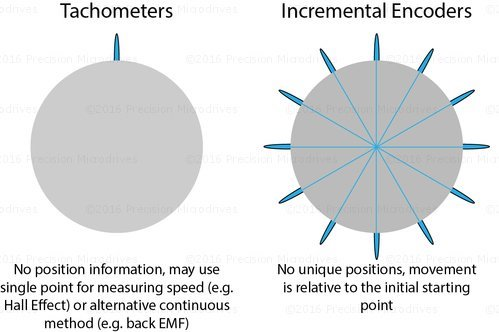
\includegraphics[width=.5\textwidth]{Controls/encoders.jpg}
  \caption{\label{fig:encoders}Tachometer vs. Rotary Encoder}
\end{figure}

However, rotary encoders have a low upper bound of approximately 10,000 for the RPM readings that they can register which might present problems at very high speeds that are to be expected during the full-scale operation of the system. On the other hand, tachometers are better suited for high speed applications as they do not suffer from the same limitation found in rotary encoders despite the reduced functionality (not being able to read position).

For design validation purposes, the team will be performing a 9 seconds drop at which the maximum calculated RPM is in the range of $5,000 RPM$. Given that this number falls within the readable range of rotary encoders, an RPM measurement device [Fig. ~\ref{fig:RPM_00}, ~\ref{fig:RPM_01}] was prototyped using a rotary encoder.

\begin{figure}[H]
 \centering
\begin{minipage}{.5\textwidth}
  \centering
  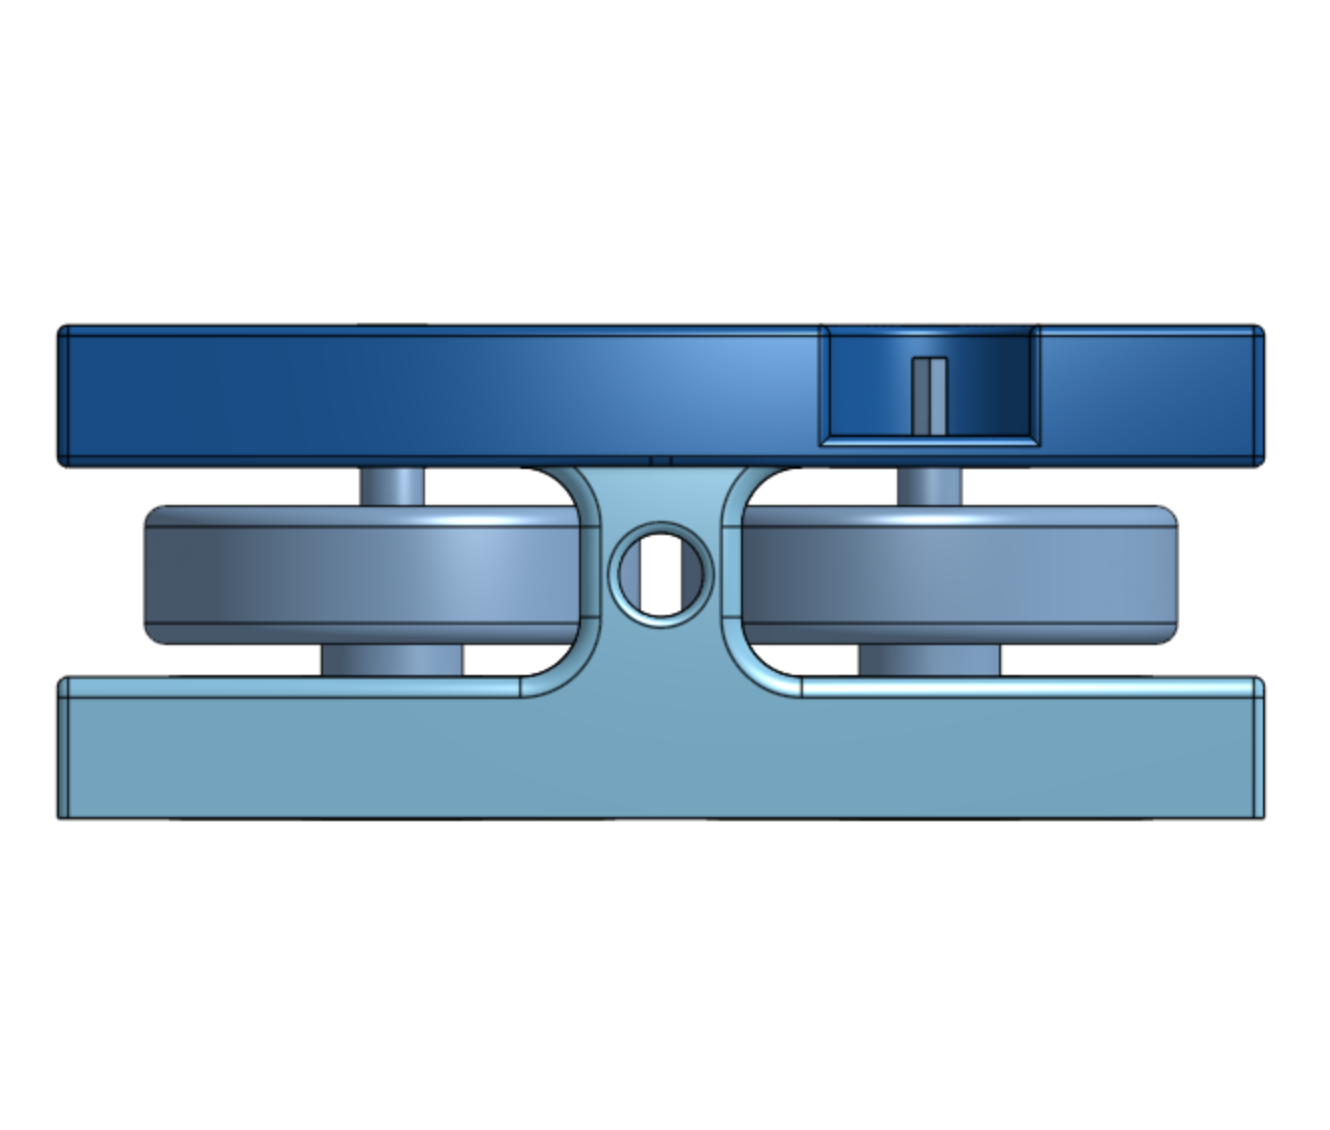
\includegraphics[width=0.8\linewidth]{Controls/RPM_00.png}
  \caption{\label{fig:RPM_00}CAD Front View} 
\end{minipage}%
\begin{minipage}{.5\textwidth}
  \centering
  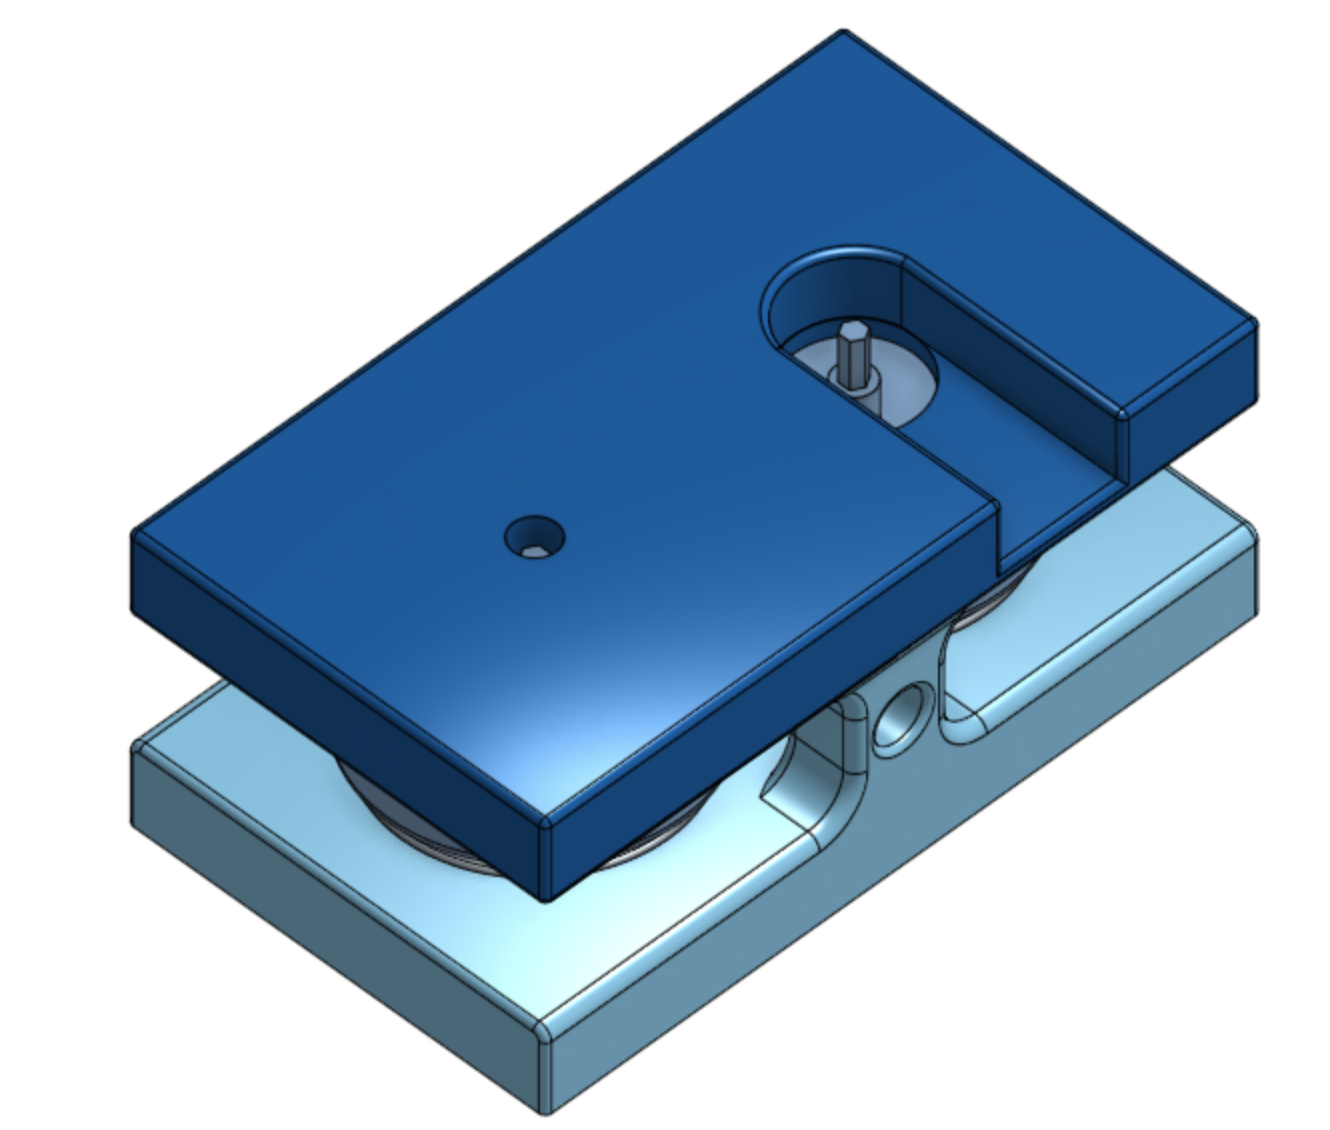
\includegraphics[width=0.8\linewidth]{Controls/RPM_01.png}
  \caption{\label{fig:RPM_01}CAD Side View}
\end{minipage}
\end{figure}

The device has two free-rotating bearings mounted side-by-side with an idler wheel mounted on top of both bearings. The tether is to be passed through the orifice that leads to the passage between the two idler wheels. A rotary encoder is installed on top of one of the idler wheels and is programmed to read the direction at which the tether is being displaced (whether it is being ejected or being pulled back) and calculations to determine the rate at which the tether is being displaced take place in the background. All this information is then relayed back to the controls unit for further processing and issuing of appropriate instructions to the motor.

As the platform design grew in complexity, the physical design of the rotary encoder had to change to accommodate. In addition, the team had opted to use an optical rotary encoder (ORE) in place of a mechanical rotary encoder since that will allow for a higher upper bound of RPM readings. The ORE that was designed uses a pair of infrared (IR) emitter/receiver LEDs that are placed co-axially across the redesigned release disks as seen in [Fig. ~\ref{fig:ORE_releaseDisks_1}] and [Fig. ~\ref{fig:ORE_releaseDisks_2}].

\begin{figure}[H]
\centering
\begin{minipage}{.5\textwidth}
  \centering
  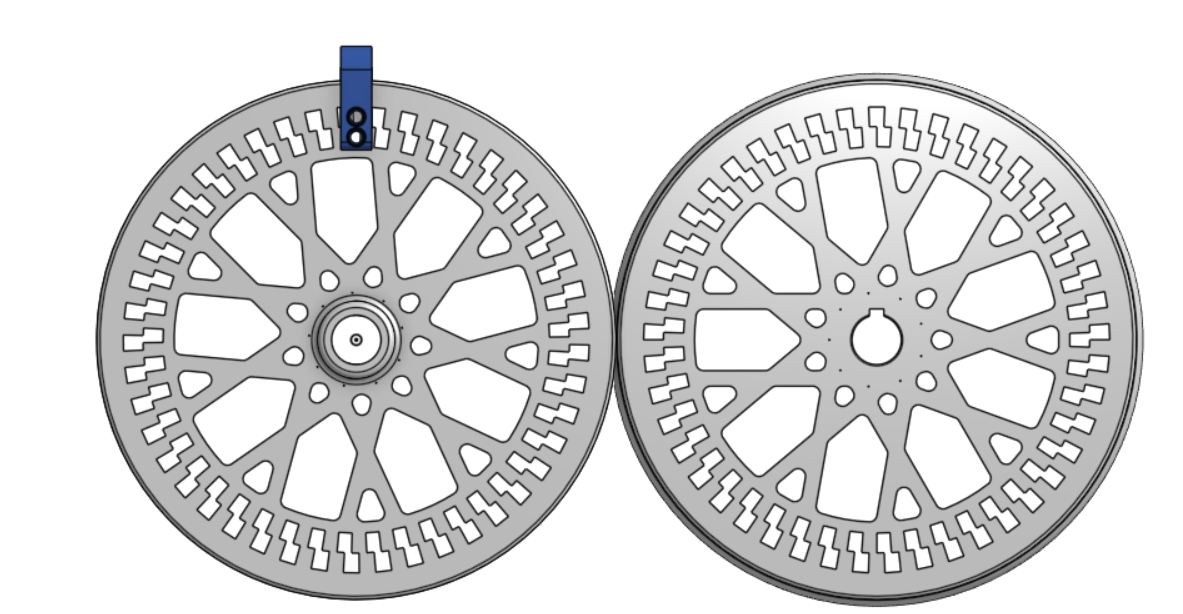
\includegraphics[width=0.9\linewidth]{Controls/ORE_releaseDisks_1.PNG}
  \caption{\label{fig:ORE_releaseDisks_1}ORE + Release Disks Front View} 
\end{minipage}%
\begin{minipage}{.5\textwidth}
  \centering
  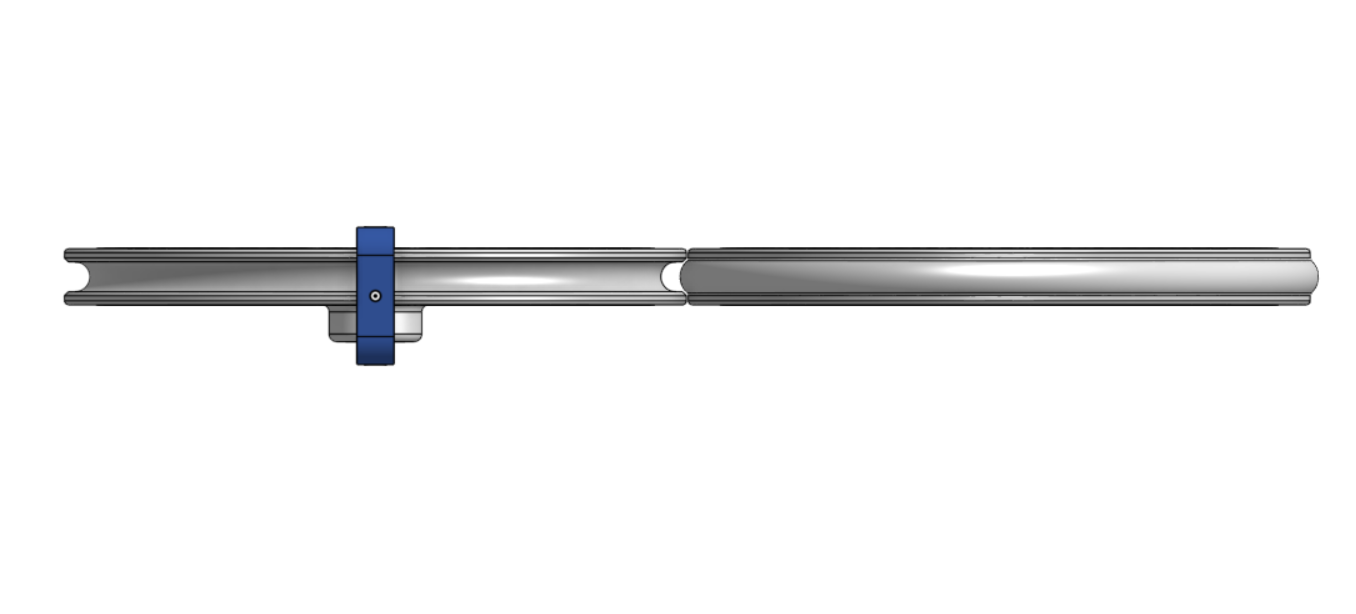
\includegraphics[width=1.0\linewidth]{Controls/ORE_releaseDisks_2.PNG}
  \caption{\label{fig:ORE_releaseDisks_2}ORE + Release Disks Top View}
\end{minipage}
\end{figure}

The ORE operates under a simple principle. Slits have an offsets such that each signal lags the other by 90\degree. This allows the MCU unit to determine the direction of rotation by comparing the current signal with the previous signal. A visual representation of the signal as seen by the MCU is shown in [Fig. ~\ref{fig:ORE_signal}]. Lastly, the schematic design used to assemble the ORE circuit is seen in [Fig. ~\ref{fig:ORE_circuit_schem}].

\begin{figure}[H]
  \centering
  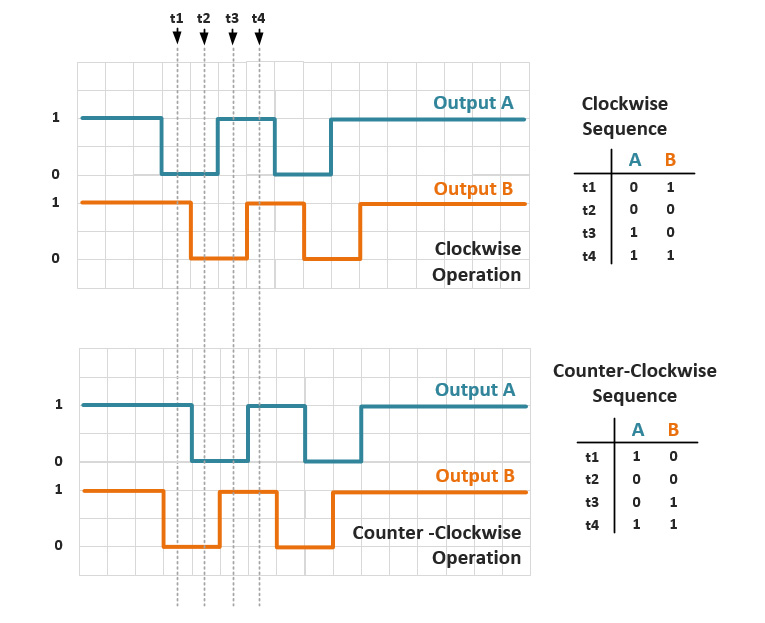
\includegraphics[width=.8\textwidth]{Controls/ORE_signal.jpg}
  \caption{\label{fig:ORE_signal}ORE Circuit Schematic}
\end{figure}

\begin{figure}[H]
  \centering
  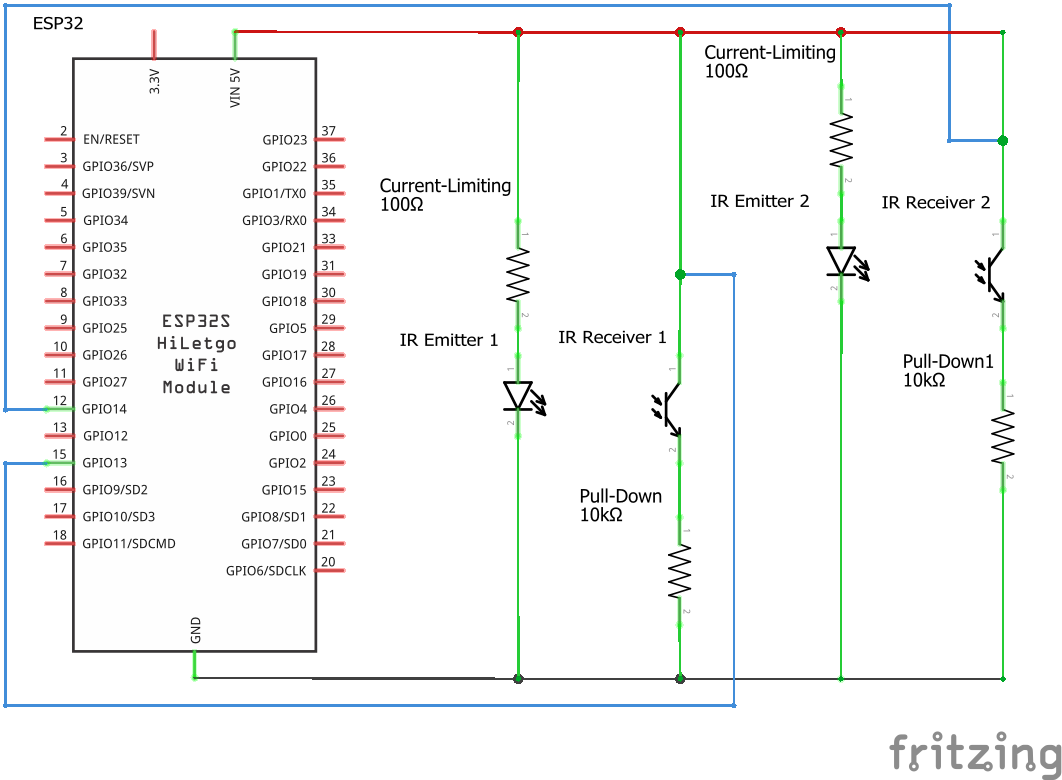
\includegraphics[width=.8\textwidth]{Controls/ORE_circuit_schem.png}
  \caption{\label{fig:ORE_circuit_schem}ORE Circuit Schematic}
\end{figure}


% ---------------------------------------------------------

\subsubsection{Controls Unit}

\begin{table}[H]
\caption{\label{tab:MCU_WRE}Weighted Ratings Evaluation of Controllers.}
\centering
\resizebox{\textwidth}{!}{%
\begin{tabular}{cc|c|P{2cm}|c|P{2cm}|c|P{2cm}|c|P{2cm}|}
\cline{3-10}
& & \multicolumn{8}{ c| }{ Concept Alternative } 				\\ \cline{3-10}
& & \multicolumn{2}{ c| }{ \cellcolor{gray!25}      RPi 3  }
& 	\multicolumn{2}{ c| }{ \cellcolor{gray!50}    Arduino  }
& 	\multicolumn{2}{ c| }{ \cellcolor{gray!75}  Teensy 3.x }
& 	\multicolumn{2}{ c| }{ \cellcolor{gray!100}  ESP32P36  } 	\\ \cline{1-10}

\multicolumn{1}{ |c  }{Criteria} &
\multicolumn{1}{ |P{2cm}| }{Importance Weight(\%)} & Rating & Weighted Rating & Rating & Weighted Rating & Rating & Weighted Rating & Rating & Weighted Rating \\ \cline{1-10}

\multicolumn{1}{ |c  }{High Clock Frequency} &
\multicolumn{1}{ |c| }{30\%} & 4 & 1.20 & 1 & 0.30 & 2 & 0.60 & 3 & 0.90 \\ \cline{1-10}

\multicolumn{1}{ |c  }{Operational Conditions Range} &
\multicolumn{1}{ |c| }{25\%} & 4 & 1.00 & 1 & 0.25 & 3 & 0.75 & 3 & 0.75 \\ \cline{1-10}

\multicolumn{1}{ |c  }{Ample GPIO Pins} &
\multicolumn{1}{ |c| }{20\%} & 4 & 0.80 & 3 & 0.60 & 2 & 0.40 & 2 & 0.40 \\ \cline{1-10}

\multicolumn{1}{ |c  }{Low Overhead} &
\multicolumn{1}{ |c| }{15\%} & 2 & 0.30 & 4 & 0.60 & 4 & 0.60 & 4 & 0.60 \\ \cline{1-10}

\multicolumn{1}{ |c  }{Ease of Programming} &
\multicolumn{1}{ |c| }{10\%} & 2 & 0.20 & 4 & 0.40 & 4 & 0.40 & 4 & 0.40 \\ \cline{1-10}

\multicolumn{1}{ |r  }{Totals} &
\multicolumn{1}{ |c| }{100\%} & & \cellcolor{gray!25}3.50 & & \cellcolor{gray!50}2.15 & & \cellcolor{gray!75}2.75 & & \cellcolor{gray!100}3.05 \\ \cline{1-10}

\end{tabular}}
\end{table}

\indent\indent The current onboard controllers consists of a mix between Arduinos and RPi’s. However, observing [Table ~\ref{tab:MCU_WRE}], it becomes clear that Arduinos are inferior and subpar to every other alternative and replacing them with a better suited product is more than justifiable. In addition, all the Arduinos currently onboard can be replaced by a single RPi 3 which is capable of interfacing all the required peripherals and sensors as it has more than ample GPIO pins and a much higher frequency than 75 Arduino Megas combined. This is owing to the fact that a RPi has a base clock frequency of 0.8GHz and can be overclocked to 1.2GHz while maintaining operational stability, whereas an Arduino Mega has a base clock frequency of 16MHz with no ability to overclock \cite{Arduino_Specs}. Moreover, the Arduino is a single core board whereas the RPi is a 4 core computer. In terms of operation, this means that an Arduino can only run one process at a time. On the other hand, the RPi can run 4 simultaneous threads, or operations, at a time.

In order to quantify such differences in operation, a benchmark was devised and used to stress test both the RPi and the Arduino. The benchmark test consisted of calculating the first 10,000 prime numbers and reporting back the execution time of the test. The benchmark was ran on the following boards using the the following configurations:

\begin{enumerate}
    \item Arduino Mega 2560 running at 16MHz
    \item RPi running at 0.8GHz (base)
    \item RPi running at 1.2GHz (OC)
\end{enumerate}

As can be observed from [Fig. ~\ref{fig:Arduino_bench}], the Arduino Mega 2560 took about 490 seconds to compute the first 10,000 prime numbers. Taking that long to compute the prime numbers can be attributed to the Arduino's low CPU frequency and its inability to multithread the operation.

\begin{figure}[H]
  \centering
  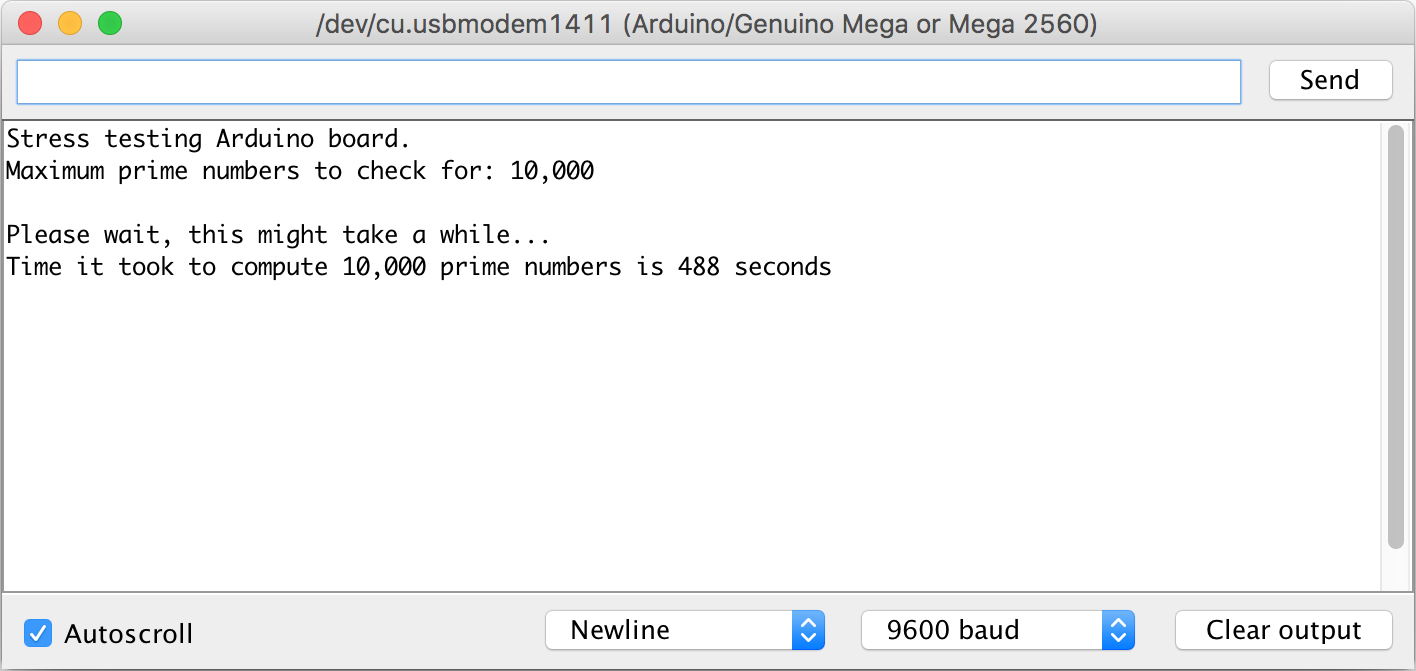
\includegraphics[width=0.85\textwidth]{Controls/Arduino_bench.png}
  \caption{\label{fig:Arduino_bench}Arduino Mega 2560 running at 16MHz}
\end{figure}

On the other end of the spectrum, the RPi was benchmarked by noting the time is took to calculate the first 10,000 prime numbers. The main difference between the RPi's benchmark and the Arduino's benchmark is that the RPi's operation was multithreaded, or in other words, the instructions to compute the prime numbers was distributed among the 4 cores of the RPi.

\begin{figure}[H]
 \centering
 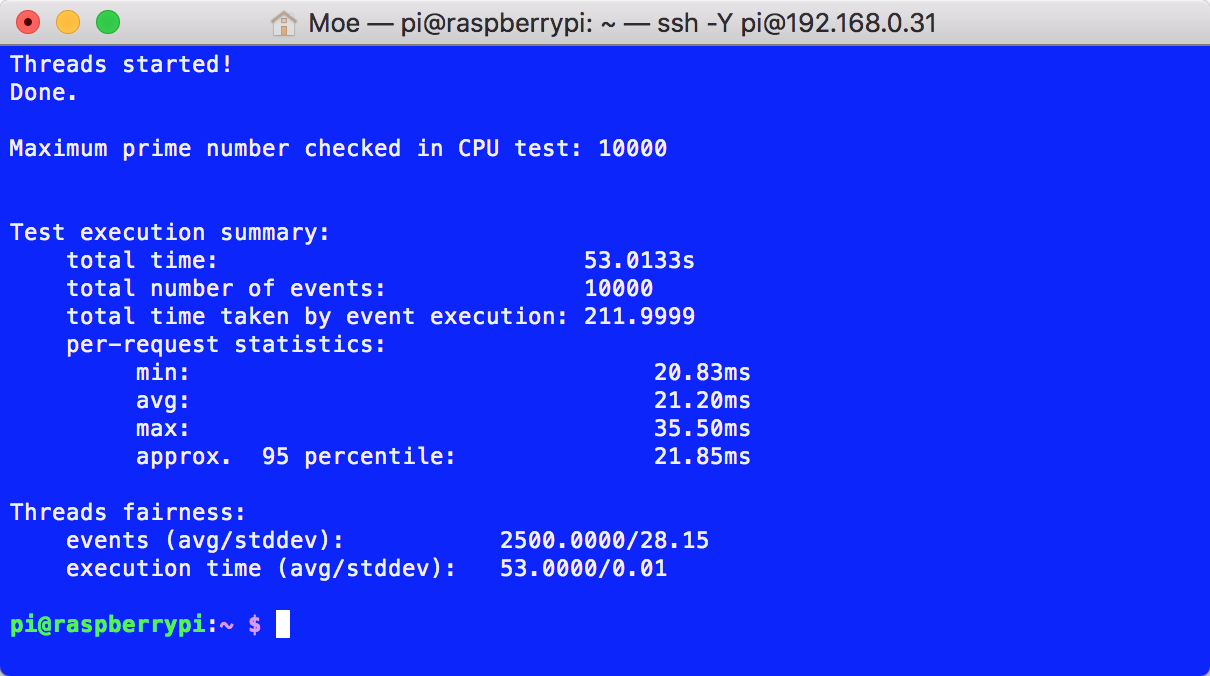
\includegraphics[width=0.85\linewidth]{Controls/RPi_Base.png}
 \caption{\label{fig:RPi_Base}RPi running at 0.8GHz (base)} 
\end{figure}

As can be observed in [Fig. ~\ref{fig:RPi_Base}], the RPi running at stock configuration was able to compute the prime numbers in about 55 seconds, almost 9 times faster than the Arduino Mega.

\begin{figure}[H]
 \centering
 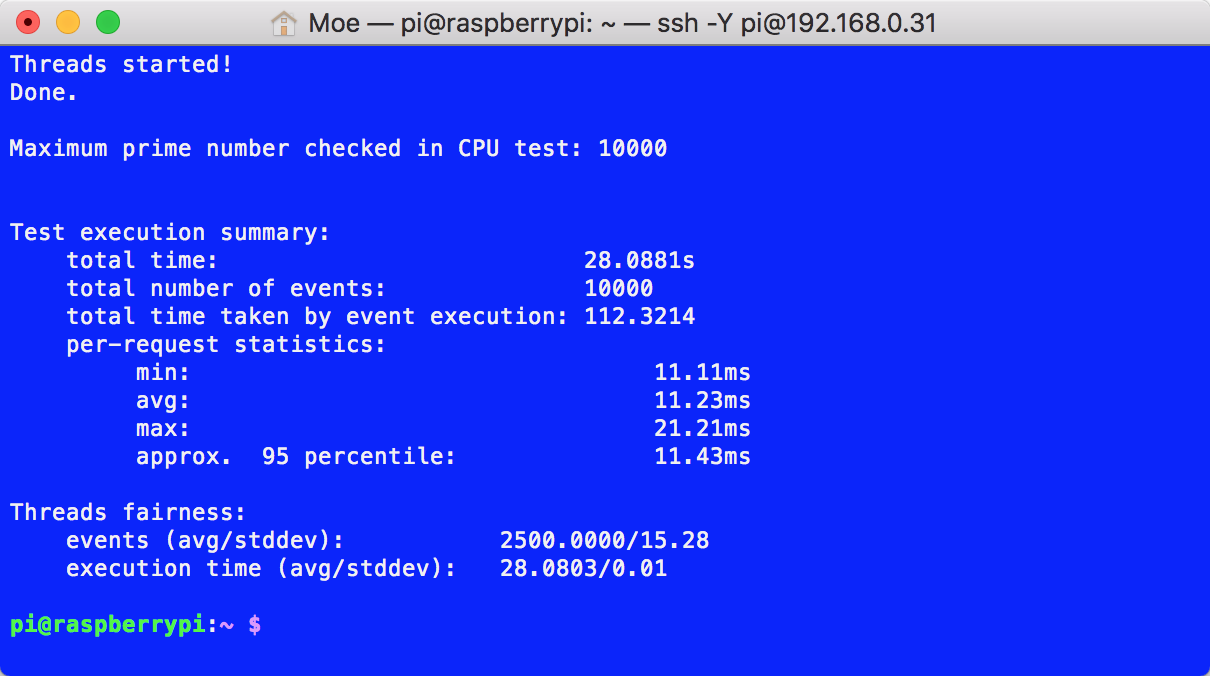
\includegraphics[width=0.85\linewidth]{Controls/RPi_OC.png}
 \caption{\label{fig:RPi_OC}RPi running at 1.2GHz (OC)}
\end{figure}

For the last benchmark, the RPi was overclocked and the benchmark was once again ran. The results are seen in [Fig. ~\ref{fig:RPi_OC}]. It took the RPi about 30 seconds, which is 16 times faster than the Arduino, and almost 2 times faster than a RPi running stock configurations.

Lastly, the overhead incurred by running an OS on the Raspberry Pi can be drastically improved upon by replacing Raspbian OS, the official distribution offered by the Raspberry Pi Foundation, with a highly optimized version of the Raspbian OS named DietPi, which is a community offered distribution.

\begin{table}[H]
\caption{\label{tab:Diet_vs_Lite}DietPi vs. Raspbian Lite.}
\centering
\begin{tabular}{l|c|c|c}
\hline\hline
General Stats  & Description	& DietPi	& Lite 	\\
\hline
Total Image Size  	& OS size. Lower is better.  			& 589MB & 1424MB 	\\\hline
Total Processes 	& Programs and services. Lower is better. 	& 11 	& 18 	\\\hline
Installed Packages  & Lower is better. 							& 265   & 406 	\\\hline
Root Filesystem    	& Lower is better. 						& 533MB & 931MB		\\\hline
System Response    	& Latency before increasing CPU. Lower is better. 	& 25 ms & 100ms \\\hline
\end{tabular}
\end{table}

The DietPi OS was compared against the Raspbian Lite OS, a stripped down version of the Raspbian Jessie OS used by the previous team, and the results were tabulated in [Table ~\ref{tab:Diet_vs_Lite}]. As it is clearly evident from the table, DietPi offers better performance in all aspects. First of all, it has a lower footprint size wise, meaning that the RPi will require less time to access critical OS components for operation. Furthermore, the system response time is 4 times faster for the DietPi OS than that of Raspbian Lite OS, this is important for real-time operation \cite{DietPi_Site}.

% ---------------------------------------------------------

\subsubsection{Programming language}

\indent\indent The previous teams had opted to use both, interpreted and compiled, types of language in their endeavor of building the first generation prototype. Python was used primarily on the control unit (the RPi) whereas C/C++ was deployed on the MCU's responsible for data acquisition. The "Weighted Rating Evaluation" process proves to be difficult to use for the purpose of aiding in determining which language should be used. As such, a different approach was devised. A program was written in both Python and C that approximates the value of $\pi$ using the Gregory-Leibniz series approximation,

\begin{equation}
	\pi=4\sum\limits_{n=0}^\infty \frac{(-1)^n}{2n+1}
    \label{eq:pi}
\end{equation}

The program was allowed to run for 100 million iterations before it was issued a command to timeout and return execution time. Both programs ran on the same RPi that is overclocked to 1.4GHz. Python 2.7+ was used whereas the C program was compiled using GCC 6.3.0. The results are found in [Fig. ~\ref{fig:py_pi}] and [Fig. ~\ref{fig:C_pi}], respectively.

\begin{figure}[H]
  \centering
  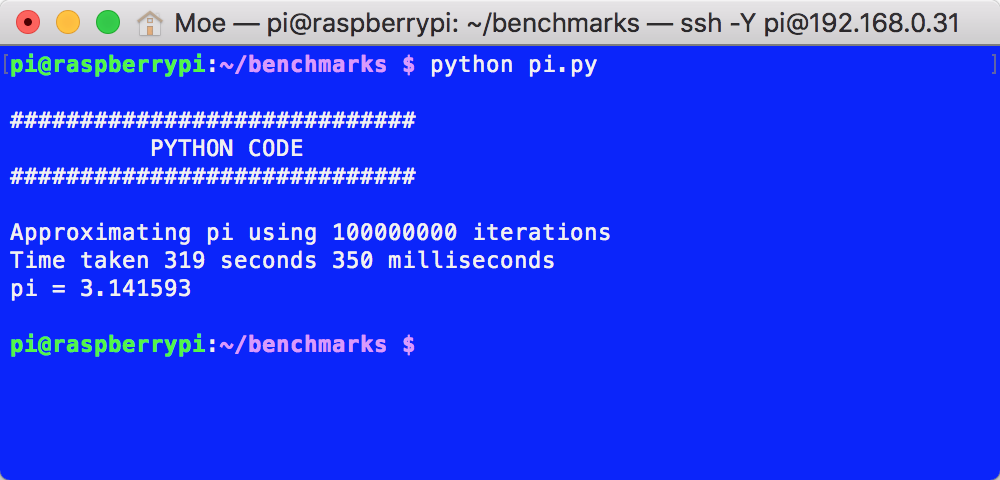
\includegraphics[width=.85\textwidth]{Controls/py_pi.png}
  \caption{\label{fig:py_pi}Execution time in Python}
\end{figure}

\begin{figure}[H]
  \centering
  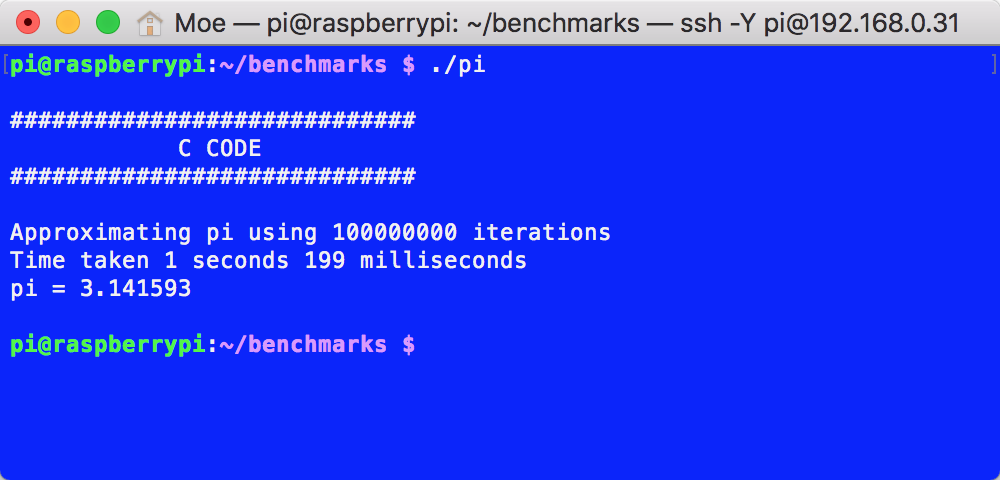
\includegraphics[width=.85\textwidth]{Controls/C_pi.png}
  \caption{\label{fig:C_pi}Execution time in C}
\end{figure}

As can be observed from the results, the Python program took approximately 320 seconds to approximate $\pi$, whereas the C program was able to approximate $\pi$ in about 1 second, 320 times faster than Python! These results are indicative that C is the obvious choice for the programming language as it is capable of delivering performance that will allow the system to operate in real-time.

